\section{Numerical Solution Procedure}\label{sec:solution}

\subsection{Time Integration Scheme}\label{subsec:time-integration-scheme}

The time integration scheme follows a simple explicit Eulerian forward procedure.
This method, however, is prone to numerical instabilities, which are often observed as alternating zick-zack like surface structures (see \autoref{sec:numerical-behavior}).
Therefore, the time step width must be limited.
As the normal or tangential displacements of a node in one step are bad measures due to the varying distances between the nodes, it was chosen to use the surface angles (which are a measure for curvature) as indicator for time step width.

The angle difference is calculated in accordance to the equations in \autoref{sec:surface-evolution} with $\Step\Shift = \dot\Shift \Step\Time$.

\begin{equation}
    \max_i^{\Nodes} \max_j^{[\Upper, \Lower]} \max_k^{[\Normal, \Tangential]} \arcsin \left( \frac{\SurfaceDistance}{\SurfaceDistance'} \sin \SurfaceVectorAngle_{jk} \right)  < \qtyrange{0.01}{0.1}{\radian}
    \label{eq:maximum-angle-difference}
\end{equation}

\subsection{Step System Solution}\label{subsec:step-system-solution}

The application of the \gls{TEP} leads to a non-linear system of equations, although most equations are linear therein with a few exceptions, most notably the main dissipation equality constraint.
The system size is dependent on the count of particles present in the simulation and the count of points defining their surface.
Typically, it contains from a few hundred to a few thousands of components.
Solution of this system is accomplished using the standard Newton method, as this method is known for fast convergence thus sparing evaluations of the system.
This method requires the evaluation of the systems gradient resp.~it's Jacobian matrix, which is sparse and follows the general structure shown in \autoref{fig:implementation/sparse_structure}.
The complete set of components for the Jacobian are given in \autoref{sec:components-of-the-lagrangian-gradients-jacobian}.
Newton's method is, however, also known for its vulnerability to the choice of the initial solution estimation (see \autoref{subsubsec:solution-estimation}).
As the regarded system only includes linear, bilinear and quadratic terms, non-convergence does not have to be expected here.
However, the system may have two solutions caused by the quadratic terms, so the procedure may converge to the wrong one.

Most notably, in a particle system without external loads, the trivial solution (overall dissipation is zero) is a valid solution of the equation system, but the minimum of dissipation rather its maximum.
During testing, it has been noticed that in cases where the solution procedure converges to the trivial solution, doubling the initial solution estimate often pushes the procedure to converge to the right solution.
This is a simple and fast trick to avoid this issue.
The reasoning behind this is, that the overall dissipation at necks is often underestimated by the step estimator.
Convergence to the trivial solution usually occurs, when the estimated overall dissipation is to small by several orders of magnitude.

The calculation of a Newton step requires the solution of the linear system in \autoref{eq:newton-step}, where $J_{\LagrangeFunction}$ is the Jacobian of the Lagrangian and $\Grad \LagrangeFunction$ it's gradient.
The system is solved in each step by LU-factorization using an algorithm specialized for sparse matrices of \textcite{Davis2006} implemented in the CSparse.NET package \textcite{Woltering2024}.

\begin{equation}
    J_{\LagrangeFunction}(x) \cdot \Step x = -\Grad \LagrangeFunction(x)
    \label{eq:newton-step}
\end{equation}

\begin{figure}
    \centering
    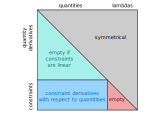
\includegraphics[scale=0.6]{img/implementation/sparse_structure}
    \caption{General Structure of the Systems Jacobian Matrix}
    \label{fig:implementation/sparse_structure}
\end{figure}

\subsubsection{Solution Estimation}\label{subsubsec:solution-estimation}

The estimation of the step solution is a crucial point to ensure fast and reliable convergence of the Newton procedure.

The solution on free surfaces is easily obtained with high precision by first estimating the vacancy concentrations using \autoref{eq:vacancy-concentration}, but expressing the chemical potential by the Gibbs energy gradient of \autoref{eq:gibbs-partial-surface-normal} as in \autoref{eq:chemical-potential-by-gibbs-gradient}.

\begin{equation}
    \Estimated{\Diff\ChemicalPotential} = \frac{\partial\GibbsEnergy}{\partial\Step_{\Normal}} \cdot \frac{2\MolarVolume}{\SurfaceDistance_{\Upper} + \SurfaceDistance_{\Lower}}
    \label{eq:chemical-potential-by-gibbs-gradient}
\end{equation}

Then the fluxes are obtained using Fick's first law (\autoref{eq:fick-first}).
By balancing the fluxes and dividing by the volume gradient, the normal displacement of a node is obtained:

\begin{equation}
    \Estimated{\Step\Shift_{\Normal}} = \left( \Flux_{\Upper} - \Flux_{\Lower} \right) \left( \frac{\partial\Volume}{\partial\Shift_{\Normal}} \right)^{-1}
    \label{eq:estimate-normal-displacement}
\end{equation}

When simulating the evolution of a single particle free in space, this estimate solves the step directly.
A single Newton step is than only needed to obtain the Lagrange multipliers.
When, however, a sinter neck is present, the situation becomes much more complicated, as the neck points feature two modes of displacement with distinct volume and energy gradients and the requirement of maintaining contact.
The issue is solved using a fixed-poit iteration procedure, whose starting point is the simple estimation described above.
The target variable is the flux between the neck node and the central grain boundary node, denoted here as $\Estimated\Flux$.

In the first approximation, the normal displacement of the neck nodes must be equal to that of the grain boundary node to fulfill contact consitions.
Then, the tangetial displacement of the neck node calculates as in \autoref{eq:estimate-neck-tangetial-displacement} using the flux balance there, with $\Flux_{\Surface}$ as the estimated flux to the adjacent surface node calculated as above and $i$ as the iteration index.

\begin{equation}
    \Estimated{\Step\Shift_{\Tangential i}} =
    \left( \Estimated{\Flux_i} - \Flux_{\Surface} - \frac{\partial\Volume}{\partial\Shift_{\Normal}} \Estimated{\Step\Shift_{\Normal i}} \right)
    \left( \frac{\partial\Volume}{\partial\Shift_{\Tangential}} \right)^{-1}
    \label{eq:estimate-neck-tangetial-displacement}
\end{equation}

With this the total dissipation on the neck node is given by:

\begin{equation}
    \Estimated{\Dissipation_i}
    = \frac{\partial\GibbsEnergy}{\partial\Shift_{\Normal}} \Estimated{\Step\Shift_{\Normal i}}
    + \frac{\partial\GibbsEnergy}{\partial\Shift_{\Tangential}} \Estimated{\Step\Shift_{\Tangential i}}
    \label{eq:estimated-neck-dissipation}
\end{equation}

Using the form of the dissipation function in \autoref{eq:dissipation-function-node} the new flux is obtained as in \autoref{eq:estimated-neck-new-flux}.
The signum term is required to support negative dissipations, which occur when the system reaches a stationary state of the surface near the neck in later stages which is characterized by small fluctuations.

\begin{equation}
    \Estimated{\Flux_{i+1}} =
    \sign \Estimated{\Dissipation_i} \cdot
    \sqrt{
        \frac{\MolarVolume{\VacancyConcentration}^\Standard}{\GasConstant\Temperature}
        \frac{\DiffusionCoefficient_{\Upper}}{\SurfaceDistance_{\Upper}}
        \Abs{\Estimated{\Dissipation_i}}
    }
    \label{eq:estimated-neck-new-flux}
\end{equation}

This flux is then inserted in the iteration again in \autoref{eq:estimate-normal-displacement} for the grain boundary nodes and \autoref{eq:estimate-neck-tangetial-displacement} for the neck node till the fixed point is reached.
